\begin{comment}
\begin{itemize}
  \item RICOH THETA V(https://theta360.com/ja/about/theta/v.html)
  \item insta 360(https://www.insta360.com/jp/product/insta360-onex2)
  \item Meeting OWL(http://meetingowl.jp/?i=nav)
  \item Collaboration in 360° Videochat: Challenges and Opportunities(https://dl.acm.org/doi/10.1145/3064663.3064707)
\end{itemize}
\end{comment}

\subsubsection*{全天球カメラ}

全天球カメラの具体例としては,RICHOのTHETA V\cite{4}が挙げられる.

THETAの裏と表には,それぞれ1枚ずつ,計2枚の魚眼レンズが
取り付けられている.本体を薄く設計することで,2つの
魚眼レンズの視差を小さくして,後述するスティッチング処理を行った際
違和感のない画像を生成することを可能にしている.

TEHTAのパノラマ画像は,以下のようにして生成される.
まず,2枚の魚眼レンズで撮影された映像それぞれについて,
通常のカメラでも行われるような基本的な画像処理と,
映像それぞれの明るさや色味が合うようにする処理を行う.
生成された2枚の画像に対し,パターンマッチングを行い,
つなぐ位置を検出する.一方で,各魚眼レンズには
特有の歪みが存在し,Thetaではその歪みを補正する処理を
行っている.この2つの操作(つなぎ処理スティッチングと呼ぶ)を行い,
2枚の画像を結合することによって全天球パノラマ映像を生成している.
(図\ref{theta1},\ref{theta2}参照)

\begin{figure}[tp]
  \centering
  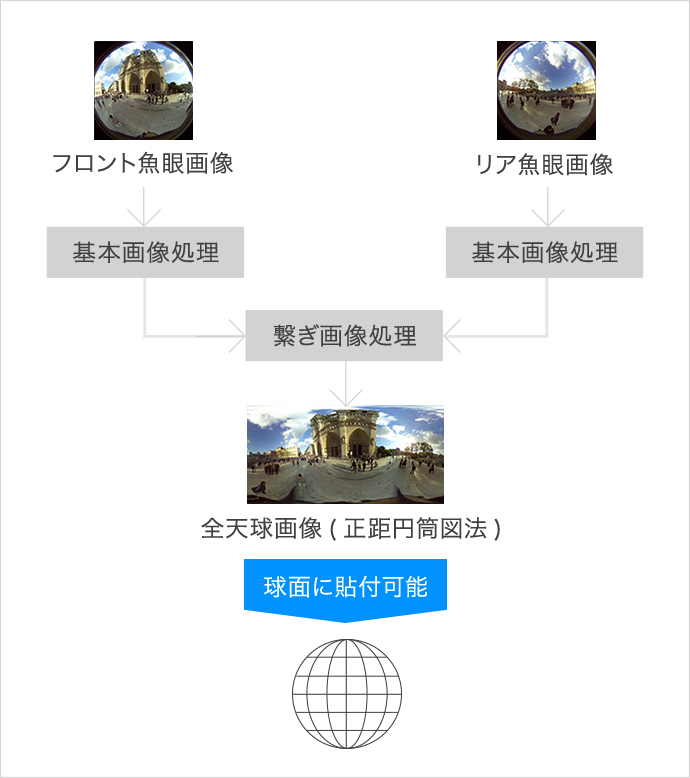
\includegraphics[scale=0.6]{fig/thetaref1.jpg}
  \caption{画像処理の流れ\cite{4}}\label{theta1}
\end{figure}

\begin{figure}[tp]
  \centering
  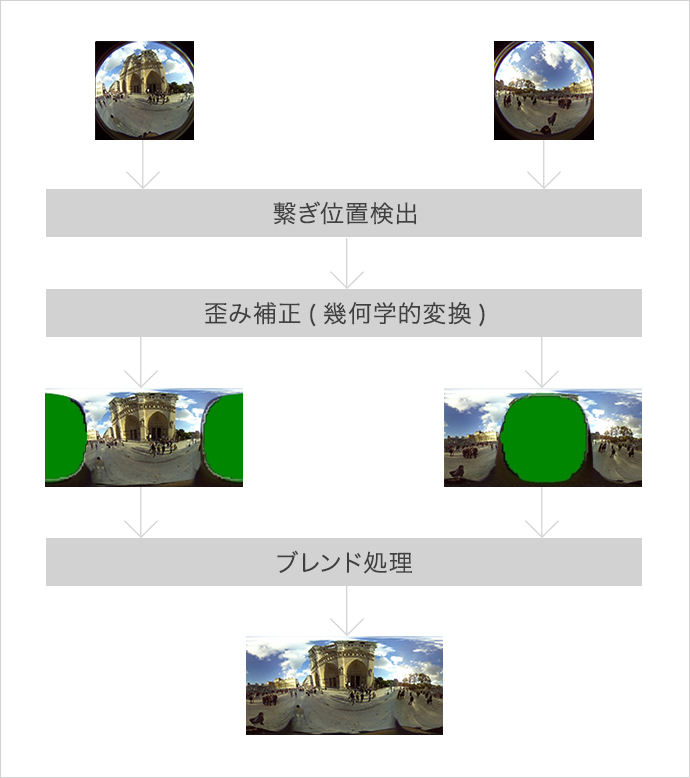
\includegraphics[scale=0.6]{fig/thetaref2.jpg}
  \caption{つなぎ処理スティッチング\cite{4}}\label{theta2}
\end{figure}

一方でパノラマ画像を生成する際に用いられる正距円筒図法であるが,
これには欠点が存在する.正距円筒図法は,球面を平面に投影する
方法の一種であり,緯線と経線が直行し,それぞれが等間隔になるように
表示された図法であり,世界地図などに広く用いられてきた.

投影の方法上,どの経線の長さも赤道の長さと一致するようになっているが
これは球面上の経線の性質と一致していない.実際,球面上では

\begin{eqnarray}
  (緯度\theta の経線の長さ):(赤道の長さ)= \cos{\theta}:1 \nonumber \\
\end{eqnarray}

であり,正距円筒図法上では,緯度$\theta$部分が横方向に$\frac{1}{cos\theta}$だけ
拡大されていることになる.この拡大によって生じた歪みを
わかりやすく示したものがテイソーの指示楕円である.(図\ref{teiso})
高緯度領域ほど,横方向に拡大されて楕円が大きくなる様子が図示されている.

\begin{figure}[tp]
  \centering
  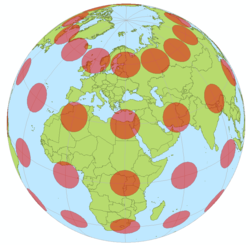
\includegraphics[scale=1.0]{fig/teiso1.png}
  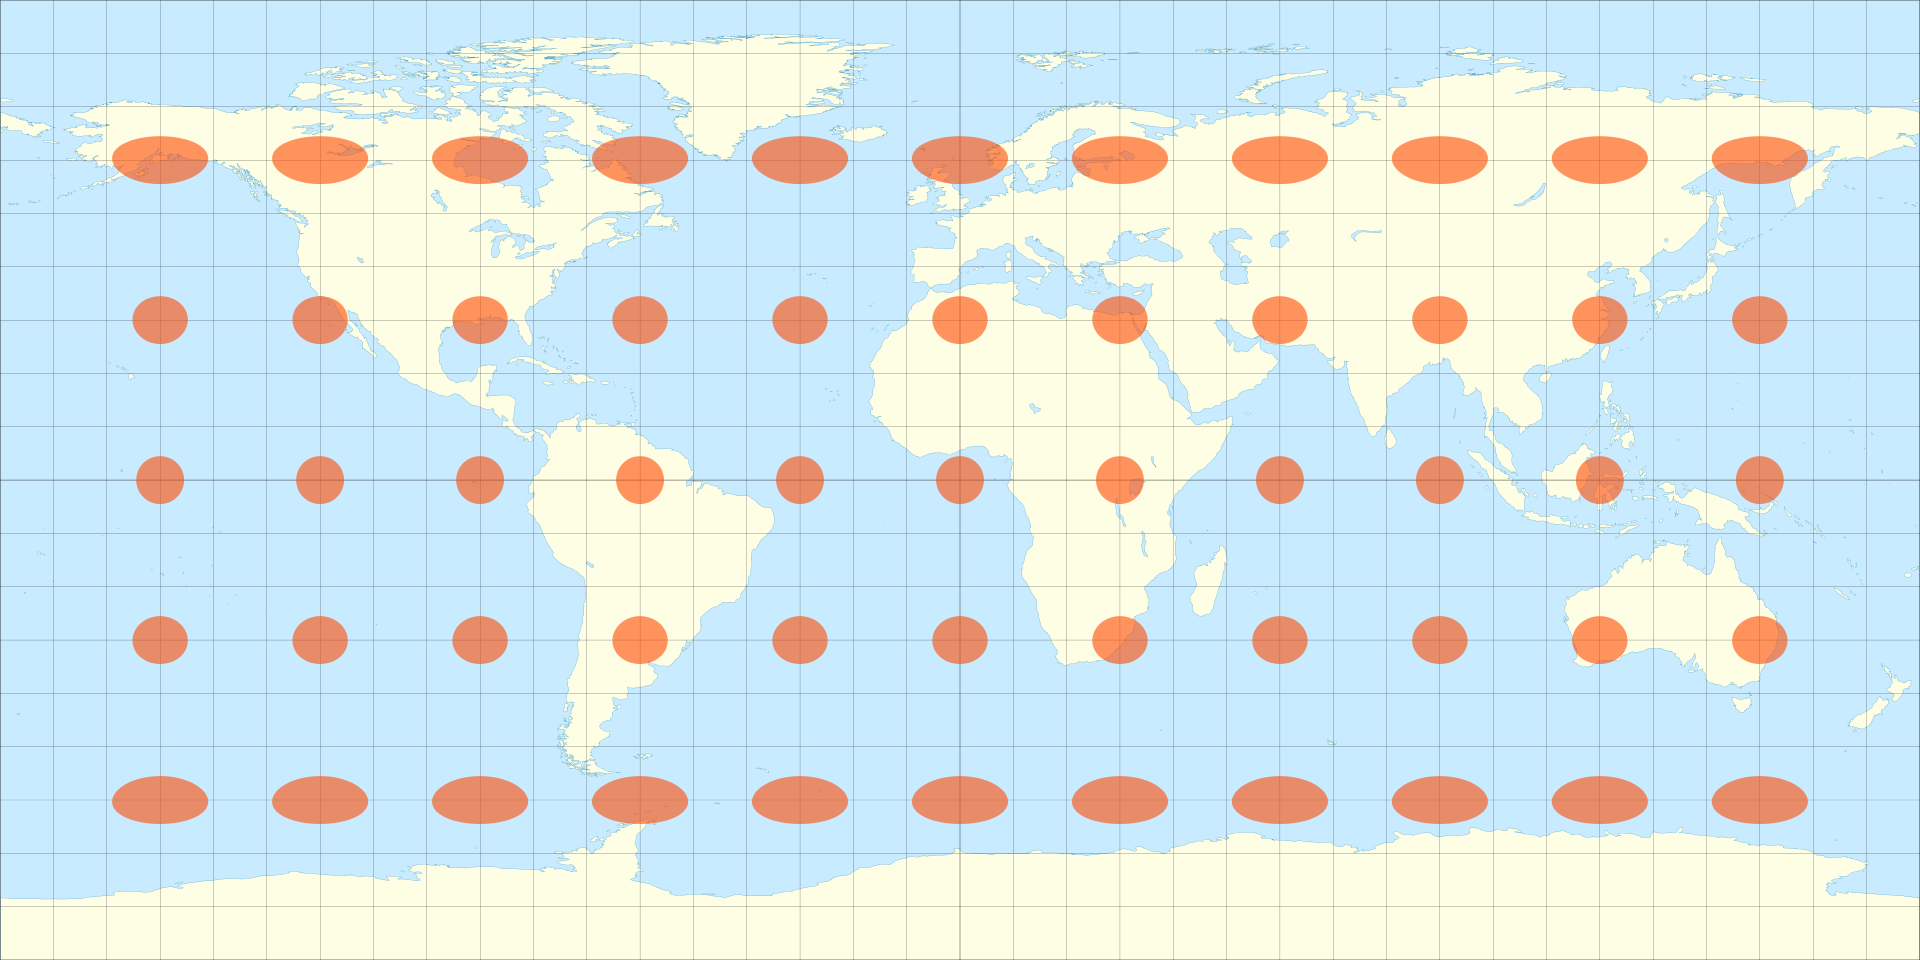
\includegraphics[scale=0.2]{fig/teiso2.png}
  \caption{テイソーの指示楕円\cite{20}}\label{teiso}
\end{figure}

全天球カメラを利用し,さらにパノラマ画像をそのまま表示するのではなく,
臨場感のあるビデオ会議を可能にしたデバイスとしてはMeetingOWL\cite{21}がある.

\begin{figure}[tp]
  \centering
  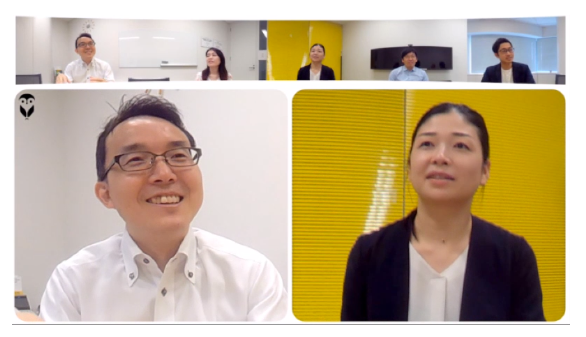
\includegraphics[scale=0.7]{fig/OWL.png}
  \caption{MeetingOWLの画面\cite{21}}
\end{figure}

\subsection*{全天球カメラの応用}

MeetingOWLは,マイクによる声の入力と,全天球映像から得られる話者の
姿勢によって,現在会話中の人物に焦点を当て,拡大して表示する
システムである.位置関係を損なわない画像の拡大により視認性が向上し,
臨場感が増している.しかし,通信相手が映像に映っている人物の誰を見ている
かについては,依然共有方法が存在していない.

全天球カメラを使用する効果に関する研究は,Tangら\cite{19}が行っている.
Tangらは,360度映像ビデオチャットアプリを作成し,それを利用して
遠隔地から現地の作業相手を支援するタスクの実験を行った.その実験の結果,
全天球カメラを用いることの利点として,以下を挙げている.

\begin{itemize}
  \item 全天球カメラの視野の広さのおかげで,カメラ位置の調整の必要が少なくなり,
  遠隔地の参加者が自由に見たい場所を見ることができるようになった.
  \item 視野の広さの影響で,遠隔地の参加者がより多くの情報を獲得でき,より
  良く作業を支援することができた.
\end{itemize}

全天球カメラは,使用者の周囲全体を映しているので,遠隔地の参加者は使用者の
周辺を自由に見渡せ,使用者の状況をすぐに知ることが出来る.一方で,全天球カメラ
の問題点として,以下を挙げている.

\begin{itemize}
  \item 遠隔地の参加者は,自由に映像を見ることが出来る一方で,現地の参加者
  と見ているものが一致しない場合があった.
  \item カメラの角度調節などを指示する際の語彙が不足していた.(カメラを上方向に
  傾ける操作を「上げる」と呼び,それがカメラを上昇させる操作と誤解される等)
\end{itemize}

ここに挙げた問題点の1つ目は,全天球カメラの視野の広さに起因するものであり,2つ目は
コミュニケーション自体が複雑化したことに起因するものである.視線情報の
共有や,3次元的な複雑な情報の直観的な表示方法を考えることが重要である.